\chapter{Aikavaativuus}

\index{aikavaativuus}

Kisakoodauksessa oleellinen asia on algoritmien tehokkuus.
Yleensä on helppoa suunnitella algoritmi,
joka ratkaisee tehtävän hitaasti,
mutta todellinen vaikeus piilee siinä,
kuinka keksiä nopeasti toimiva algoritmi.
Jos algoritmi on liian hidas, se tuottaa vain
osan pisteistä tai ei pisteitä lainkaan.

Aikavaativuus (\textit{time complexity}) on kätevä tapa arvioida,
kuinka nopeasti algoritmi toimii.
Se arvioi algoritmin tehokkuutta funktiona,
jonka parametrina on syötteen koko.
Aikavaativuuden avulla algoritmista voi päätellä ennen koodaamista,
onko se riittävän tehokas tehtävän ratkaisuun.

\section{Laskusäännöt}

Algoritmin aikavaativuus merkitään $O(\cdots)$,
jossa kolmen pisteen tilalla
on kaava, joka kuvaa algoritmin ajankäyttöä.
Yleensä muuttuja $n$ esittää syötteen kokoa.
Esimerkiksi jos algoritmin syötteenä on taulukko lukuja,
$n$ on lukujen määrä,
ja jos syötteenä on merkkijono,
$n$ on merkkijonon pituus.

\subsubsection*{Silmukat}

Algoritmin ajankäyttö johtuu usein
pohjimmiltaan silmukoista,
jotka käyvät syötettä läpi.
Mitä enemmän sisäkkäisiä silmukoita
algoritmissa on, sitä hitaampi se on.
Jos sisäkkäisiä silmukoita on $k$,
aikavaativuus on $O(n^k)$.

Esimerkiksi seuraavan koodin aikavaativuus on $O(n)$:
\begin{lstlisting}
for (int i = 1; i <= n; i++) {
    // koodia
}
\end{lstlisting}

Vastaavasti seuraavan koodin aikavaativuus on $O(n^2)$:
\begin{lstlisting}
for (int i = 1; i <= n; i++) {
    for (int j = 1; j <= n; j++) {
        // koodia
    }
}
\end{lstlisting}

\subsubsection*{Suuruusluokka}

Aikavaativuus ei kerro tarkasti,
montako kertaa silmukan sisällä oleva koodi suoritetaan,
vaan se kertoo vain suuruusluokan.
Esimerkiksi seuraavissa esimerkeissä silmukat
suoritetaan $3n$, $n+5$ ja $\lfloor n/2 \rfloor$ kertaa,
mutta kunkin koodin aikavaativuus on sama $O(n)$.

\begin{lstlisting}
for (int i = 1; i <= 3*n; i++) {
    // koodia
}
\end{lstlisting}

\begin{lstlisting}
for (int i = 1; i <= n+5; i++) {
    // koodia
}
\end{lstlisting}

\begin{lstlisting}
for (int i = 1; i <= n; i += 2) {
    // koodia
}
\end{lstlisting}

Seuraavan koodin aikavaativuus on $O(n^2)$,
koska silmukoiden sisällä oleva
koodi suoritetaan $1+2+\cdots+n = \frac{n(n+1)}{2}$ kertaa.

\begin{lstlisting}
for (int i = 1; i <= n; i++) {
    for (int j = 1; j <= i; j++) {
        // koodia
    }
}
\end{lstlisting}

\subsubsection*{Peräkkäisyys}

Jos koodissa on peräkkäisiä osia,
kokonaisaikavaativuus on suurin yksittäisen
osan aikavaativuus.
Tämä johtuu siitä, että koodin hitain
vaihe on yleensä koodin pullonkaula
ja muiden vaiheiden merkitys on pieni.

Esimerkiksi seuraava koodi muodostuu
kolmesta osasta,
joiden aikavaativuudet ovat $O(n)$, $O(n^2)$ ja $O(n)$.
Niinpä koodin aikavaativuus on $O(n^2)$.

\begin{lstlisting}
for (int i = 1; i <= n; i++) {
    // koodia
}
for (int i = 1; i <= n; i++) {
    for (int j = 1; j <= n; j++) {
        // koodia
    }
}
for (int i = 1; i <= n; i++) {
    // koodia
}
\end{lstlisting}

\subsubsection*{Monta muuttujaa}

Joskus syötteessä on monta muuttujaa,
jotka vaikuttavat aikavaativuuteen.
Tällöin myös aikavaativuuden kaavassa esiintyy
monta muuttujaa.

Esimerkiksi seuraavan koodin
aikavaativuus on $O(nm)$:

\begin{lstlisting}
for (int i = 1; i <= n; i++) {
    for (int j = 1; j <= m; j++) {
        // koodia
    }
}
\end{lstlisting}

\subsubsection*{Rekursio}

Rekursiivisen funktion aikavaativuuden
määrittää, montako kertaa funktiota kutsutaan yhteensä
ja mikä on yksittäisen kutsun aikavaativuus.
Kokonais\-aikavaativuus saadaan kertomalla
nämä arvot toisillaan.

Tarkastellaan esimerkiksi seuraavaa funktiota:

\begin{lstlisting}
void f(int n) {
    if (n == 1) return;
    f(n-1);
}
\end{lstlisting}
Kutsu $\texttt{f}(n)$ aiheuttaa yhteensä $n$ funktiokutsua,
ja jokainen funktiokutsu vie vakioajan,
joten aikavaativuus on $O(n)$.

Tarkastellaan sitten seuraavaa funktiota:

\begin{lstlisting}
void g(int n) {
    if (n == 1) return;
    g(n-1);
    g(n-1);
}
\end{lstlisting}

Tässä tapauksessa funktio haarautuu kahteen osaan,
joten kutsu $\texttt{g}(n)$ aiheuttaa kaikkiaan seuraavat kutsut:

\begin{center}
\begin{tabular}{rr}
kutsu & kerrat \\
\hline
$\texttt{g}(n)$ & 1 \\
$\texttt{g}(n-1)$ & 2 \\
$\texttt{g}(n-2)$ & 4 \\
$\cdots$ & $\cdots$ \\
$\texttt{g}(1)$ & $2^{n-1}$ \\

\end{tabular}
\end{center}

Tämän perusteella kutsun $\texttt{g}(n)$ aikavaativuus on

\[1+2+4+\cdots+2^{n-1} = 2^n-1 = O(2^n).\]

\section{Vaativuusluokkia}

\index{vaativuusluokka}

\subsubsection*{$O(1)$ (vakioaikainen)}

Aikavaativuus $O(1)$ tarkoittaa,
että algoritmi on vakioaikainen
eli algoritmin nopeus ei riipu syötteen koosta.
Tyypillinen $O(1)$-algoritmi on suora kaava
vastauksen laskemiseen.

\subsubsection*{$O(\log n)$ (logaritminen)}

Logaritminen aikavaativuus $O(\log n)$
syntyy usein siitä, että algoritmi
puolittaa syötteen koon joka askeleella.
Logaritmi $\log_2 n$ näet ilmaisee, montako
kertaa luku $n$ täytyy puolittaa,
ennen kuin tuloksena on 1.

\subsubsection*{$O(\sqrt n)$ (neliöjuuri)}

Aikavaativuus $O(\sqrt n)$ sijoittuu
vaativuuksien $O(\log n)$ ja $O(n)$ välimaastoon.
Neliöjuuren erityinen ominaisuus on,
että $\sqrt n = n/\sqrt n$, joten neliöjuuri
osuu tietyllä tavalla syötteen puoliväliin.

\subsubsection*{$O(n)$ (lineaarinen)}

Lineaarinen algoritmi käy syötteen läpi
kiinteän määrän kertoja.
Tämä on usein paras mahdollinen aikavaativuus,
koska yleensä syöte täytyy käydä
läpi ainakin kerran,
ennen kuin algoritmi voi ilmoittaa vastauksen.

\subsubsection*{$O(n \log n)$ (järjestäminen)}

Aikavaativuus $O(n \log n)$ viittaa usein
syötteen järjestämiseen,
koska tehokkaat järjestämisalgoritmit toimivat
ajassa $O(n \log n)$.
Toinen mahdollisuus on, että algoritmi
käyttää tietorakennetta,
jonka operaatiot ovat $O(\log n)$-aikaisia.

\subsubsection*{$O(n^2)$ (neliöllinen)}

Neliöllinen aikavaativuus $O(n^2)$ voi syntyä
siitä, että algoritmissa on 
kaksi sisäkkäistä silmukkaa.
Neliöllinen algoritmi voi käydä läpi kaikki
tavat valita joukosta kaksi alkiota.

\subsubsection*{$O(n^3)$ (kuutiollinen)}

Kuutiollinen aikavaativuus $O(n^3)$ voi syntyä siitä,
että algoritmissa on 
kolme sisäkkäistä silmukkaa.
Kuutiollinen algoritmi voi käydä läpi kaikki
tavat valita joukosta kolme alkiota.

\subsubsection*{$O(2^n)$ (osajoukot)}

Aikavaativuus $O(2^n)$ tarkoittaa usein,
että algoritmi käy läpi kaikki syötteen osajoukot.
Esimerkiksi joukon $\{1,2,3\}$ osajoukot ovat
$\emptyset$, $\{1\}$, $\{2\}$, $\{3\}$, $\{1,2\}$,
$\{1,3\}$, $\{2,3\}$, $\{1,2,3\}$,
missä $\emptyset$ on tyhjä joukko.

\subsubsection*{$O(n!)$ (permutaatiot)}

Aikavaativuus $O(n!)$ voi syntyä siitä,
että algoritmi käy läpi kaikki syötteen permutaatiot.
Esimerkiksi joukon $\{1,2,3\}$ permutaatiot ovat
$(1,2,3)$, $(1,3,2)$, $(2,1,3)$, $(2,3,1)$,
$(3,1,2)$ sekä $(3,2,1)$.

~\\
\noindent
Algoritmi on \textit{polynominen},
jos sen aikavaativuus on korkeintaan $O(n^k)$,
kun $k$ on vakio.
Edellä mainituista aikavaativuuksista
kaikki paitsi $O(2^n)$ ja $O(n!)$
ovat polynomisia.
Käytännössä vakio $k$ on yleensä pieni,
minkä ansiosta
polynomisuus kuvastaa sitä,
että algoritmi on tehokas.

Useimmat tässä kirjassa esitettävät algoritmit
ovat polynomisia.
Silti on paljon ongelmia, joihin ei tunneta
polynomista algoritmia eli ei mitään tehokasta
ratkaisutapaa.
Esimerkiksi NP-ongelmien joukko sisältää monia 
tärkeitä ongelmia,
joihin ei tiedetä polynomista algoritmia.

\section{Tehokkuuden arviointi}

Aikavaativuuden hyötynä on,
että sen avulla voi arvioida ennen algoritmin
toteuttamista, onko algoritmi riittävän nopea
tehtävän ratkaisemiseen.
Lähtökohtana arviossa on, että nykyaikainen tietokone
pystyy suorittamaan sekunnissa sadasta miljoonasta
miljardiin koodissa olevaa komentoa.

Oletetaan esimerkiksi, että tehtävän aikaraja on 
yksi sekunti ja syötteen koko on $n=10^5$.
Jos algoritmin aikavaativuus on $O(n^2)$,
algoritmi suorittaa noin $(10^5)^2=10^{10}$ komentoa.
Tähän kuluu aikaa ainakin kymmenen sekunnin luokkaa,
joten algoritmi vaikuttaa liian hitaalta tehtävän ratkaisemiseen.

Käänteisesti syötteen koosta voi päätellä,
kuinka tehokasta algoritmia tehtävän laatija odottaa
ratkaisijalta.
Seuraavassa taulukossa on joitakin hyödyllisiä arvioita,
jotka olettavat, että tehtävän aikaraja on yksi sekunti.

\begin{center}
\begin{tabular}{ll}
syötteen koko ($n$) & haluttu aikavaativuus \\
\hline
$n \le 10^{18}$ & $O(1)$ tai $O(\log n)$ \\
$n \le 10^{12}$ & $O(\sqrt n)$ \\
$n \le 10^6$ & $O(n)$ tai $O(n \log n)$ \\
$n \le 5000$ & $O(n^2)$ \\
$n \le 500$ & $O(n^3)$ \\
$n \le 25$ & $O(2^n)$ \\
$n \le 10$ & $O(n!)$ \\
\end{tabular}
\end{center}

Esimerkiksi jos syötteen koko on $n=10^5$,
tehtävän laatija odottaa luultavasti
algoritmia, jonka aikavaativuus on $O(n)$ tai $O(n \log n)$.
Tämä tieto helpottaa algoritmin suunnittelua,
koska se rajaa pois monia lähestymistapoja,
joiden tuloksena olisi hitaampi aikavaativuus.

Aikavaativuus ei kerro kuitenkaan kaikkea algoritmin
tehokkuudesta, koska se kätkee toteutuksessa olevat
vakiokertoimet. Esimerkiksi aikavaativuuden $O(n)$
algoritmi voi tehdä käytännössä $n/2$ tai $5n$ operaatiota.
Tällä on merkittävä vaikutus algoritmin
todelliseen ajankäyttöön.

\section{Suurin alitaulukko}

\index{suurin alitaulukko}

Yleensä ohjelmointitehtävän ratkaisuun on monta
luontevaa algoritmia, joiden aikavaativuudet eroavat.
Tutustumme seuraavaksi klassiseen ongelmaan,
jonka suoraviivaisen ratkaisun aikavaativuus on $O(n^3)$,
mutta algoritmia parantamalla aikavaativuudeksi
tulee ensin $O(n^2)$ ja lopulta $O(n)$.

\begin{task}
Annettuna on taulukko, jossa on $n$ kokonaislukua.
Tehtäväsi on etsiä alitaulukko (taulukon yhtenäinen väli),
jonka lukujen summa on mahdollisimman suuri.
\end{task}

Tehtävän kiinnostavuus on siinä, että taulukossa
saattaa olla negatiivisia lukuja.
Vaikka negatiiviset luvut pienentävät summaa,
niitä kannattaa joskus ottaa mukaan ratkaisuun,
koska negatiivisen luvun kummallakin puolella voi
olla positiivisia lukuja, jotka kumoavat negatiivisen
luvun vaikutuksen.

Esimerkiksi taulukossa


\begin{center}
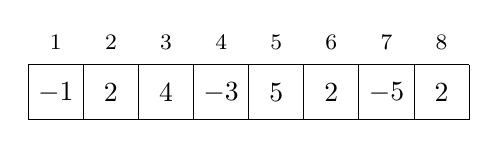
\begin{tikzpicture}[scale=0.7]
\draw (0,0) grid (8,1);

\node at (0.5,0.5) {$-1$};
\node at (1.5,0.5) {$2$};
\node at (2.5,0.5) {$4$};
\node at (3.5,0.5) {$-3$};
\node at (4.5,0.5) {$5$};
\node at (5.5,0.5) {$2$};
\node at (6.5,0.5) {$-5$};
\node at (7.5,0.5) {$2$};

\footnotesize
\node at (0.5,1.4) {$1$};
\node at (1.5,1.4) {$2$};
\node at (2.5,1.4) {$3$};
\node at (3.5,1.4) {$4$};
\node at (4.5,1.4) {$5$};
\node at (5.5,1.4) {$6$};
\node at (6.5,1.4) {$7$};
\node at (7.5,1.4) {$8$};
\end{tikzpicture}
\end{center}

optimiratkaisu on valita alitaulukko seuraavasti:

\begin{center}
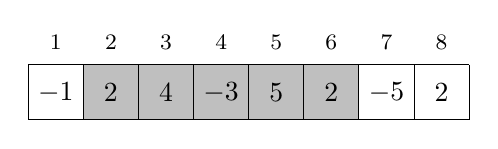
\begin{tikzpicture}[scale=0.7]
\fill[color=lightgray] (1,0) rectangle (6,1);
\draw (0,0) grid (8,1);

\node at (0.5,0.5) {$-1$};
\node at (1.5,0.5) {$2$};
\node at (2.5,0.5) {$4$};
\node at (3.5,0.5) {$-3$};
\node at (4.5,0.5) {$5$};
\node at (5.5,0.5) {$2$};
\node at (6.5,0.5) {$-5$};
\node at (7.5,0.5) {$2$};

\footnotesize
\node at (0.5,1.4) {$1$};
\node at (1.5,1.4) {$2$};
\node at (2.5,1.4) {$3$};
\node at (3.5,1.4) {$4$};
\node at (4.5,1.4) {$5$};
\node at (5.5,1.4) {$6$};
\node at (6.5,1.4) {$7$};
\node at (7.5,1.4) {$8$};
\end{tikzpicture}
\end{center}

Tämän alitaulukon lukujen summa on $2+4+(-3)+5+2=10$,
joka on suurin mahdollinen.
Keskellä oleva negatiivinen luku $-3$ kannattaa
ottaa mukaan, koska sen kummallakin puolella olevat
luvut kasvattavat summaa yli $3$:lla.

\subsubsection{Ratkaisu 1 ($O(n^3)$)}

Suoraviivainen ratkaisu tehtävään on käydä
läpi kaikki tavat valita alitaulukko taulukosta,
laskea jokaisesta vaihtoehdosta lukujen summa
ja pitää muistissa suurinta summaa.
Seuraava koodi toteuttaa tämän algoritmin:

\begin{lstlisting}
int p = 0;
for (int a = 1; a <= n; a++) {
    for (int b = a; b <= n; b++) {
        int s = 0;
        for (int c = a; c <= b; c++) {
            s += t[c];
        }
        p = max(p,s);
    }
}
cout << p << "\n";
\end{lstlisting}

Koodi olettaa, että luvut on tallennettu taulukkoon \texttt{t},
jota indeksoidaan $1 \ldots n$.
Muuttujat $a$ ja $b$ valitsevat alitaulukon ensimmäisen
ja viimeisen luvun, ja alitaulukon summa lasketaan muuttujaan $s$.
Muuttujassa $p$ on taas paras haun aikana löydetty summa.

Algoritmin aikavaativuus on $O(n^3)$, koska siinä on kolme
sisäkkäistä silmukkaa ja jokainen silmukka käy läpi $O(n)$ lukua.

\subsubsection{Ratkaisu 2 ($O(n^2)$)}

Äskeistä ratkaisua on helppoa tehostaa hankkiutumalla
eroon sisimmästä silmukasta.
Tämä on mahdollista laskemalla summaa samalla,
kun alitaulukon oikea reuna liikkuu eteenpäin.
Tuloksena on seuraava koodi:

\begin{lstlisting}
int p = 0;
for (int a = 1; a <= n; a++) {
    int s = 0;
    for (int b = a; b <= n; b++) {
        s += t[b];
        p = max(p,s);
    }
}
cout << p << "\n";
\end{lstlisting}

Tämän muutoksen jälkeen koodin aikavaativuus on $O(n^2)$,
koska siinä on kaksi sisäkkäistä silmukkaa.

\subsubsection{Ratkaisu 3 ($O(n)$)}

Yllättävää kyllä, tehtävään on olemassa myös
$O(n)$-aikainen ratkaisu eli koodista pystyy
karsimaan vielä yhden silmukan.
Ratkaisun ideana on laskea taulukon jokaiseen
kohtaan, mikä on suurin mahdollinen summa
kyseiseen kohtaan päättyvässä alitaulukossa,
ja valita suurin näistä summista.

Kun alitaulukon loppukohta $k$ on valittu,
sen muodostamiseen on kaksi vaihtoehtoa.
Yksi mahdollisuus on, että alitaulukossa
on vain yksi luku: kohdassa $k$ oleva luku.
Muussa tapauksessa siinä on ensin
kohtaan $k-1$ päättyvä alitaulukko,
johon on yhdistetty kohdassa $k$ oleva luku.

Koska tavoitteena on saada aikaan mahdollisimman
suuri summa, jälkimmäisessä tapauksessa myös
kohtaan $k-1$ päättyvä alitaulukko tulee valita niin,
että sen summa on mahdollisimman suuri.
Niinpä tehokas ratkaisu syntyy käymällä läpi
kaikki loppukohdat $k$ järjestyksessä.

Seuraava koodi toteuttaa ratkaisun:

\begin{lstlisting}
int p = 0, s = 0;
for (int k = 1; k <= n; k++) {
    s = max(t[k],s+t[k]);
    p = max(p,s);
}
cout << p << "\n";
\end{lstlisting}

Algoritmissa on vain yksi silmukka,
joka käy läpi taulukon luvut,
joten sen aikavaativuus on $O(n)$.
Tämä on myös paras mahdollinen aikavaativuus,
koska minkä tahansa algoritmin täytyy käydä
läpi ainakin kerran taulukon sisältö.

\subsubsection{Tehokkuusvertailu}

On kiinnostavaa tutkia, kuinka tehokkaita algoritmit
ovat käytännössä.
Seuraava taulukko näyttää, kuinka nopeasti äskeiset
ratkaisut toimivat eri $n$:n arvoilla
(testikoneena Intel Core i7-2677M, 1{,}80 GHz).

Jokainen syöte on muodostettu satunnaisesti,
ja taulukon luvut ovat välillä $-10^9 \ldots 10^9$.
Ajankäyttöön ei ole laskettu syötteen lukemiseen
kuluvaa aikaa.

\begin{center}
\begin{tabular}{rrrr}
taulukon koko $n$ & ratkaisu 1 & ratkaisu 2 & ratkaisu 3 \\
\hline
$10^2$ & $0{,}0$ s & $0{,}0$ s & $0{,}0$ s \\
$10^3$ & $0{,}1$ s & $0{,}0$ s & $0{,}0$ s \\
$10^4$ & > $10,0$ s & $0{,}1$ s & $0{,}0$ s \\
$10^5$ & > $10,0$ s & $5{,}3$ s & $0{,}0$ s \\
$10^6$ & > $10,0$ s & > $10,0$ s & $0{,}0$ s \\
$10^7$ & > $10,0$ s & > $10,0$ s & $0{,}0$ s \\
\end{tabular}
\end{center}

Vertailu osoittaa,
että pienillä syötteillä kaikki algoritmit
ovat tehokkaita,
mutta suuremmat syötteet tuovat esille
huomattavia eroja algoritmien suoritusajassa.
$O(n)$-aikainen ratkaisu 3 on ainoa,
joka pystyy ratkaisemaan kaikki syötteet
alle 10 sekunnissa.